\label{sec:vis}

To enable the transparent visualization, we require an ordered list of fragments for each screen pixel. 
This list of fragments is also commonly referred as an A-buffer. 
We implemented the A-buffer using per-pixel linked lists~\cite{yang2010real}. 
In our case, the A-buffer fragments represent three types of surface patches analytically computed for a given ray.

\subsection{Ray-casting}
\label{sec:spherical-patches}
To form fragments of each surface patch we employ a ray-casting technique.
To reach high performance, the ray-patch intersection is computed analytically.
For each patch, we compute a tight oriented bounding box (OBB) which we project onto the image as a splat (Fig.~\ref{fig:obb}).
This way, we lower the number of intersection tests that will be performed.

\begin{figure}[htp]
  \centering
  \begin{subfigure}[t]{0.48\columnwidth}
    \centering
    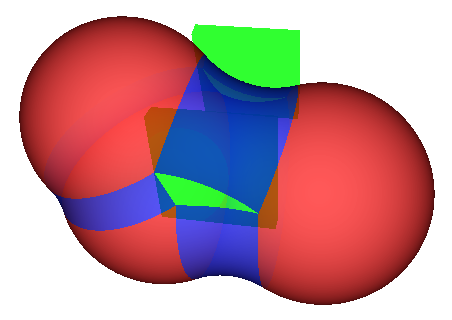
\includegraphics[width=1.5in]{image/obb-triangles.png}
  \end{subfigure}%
  \quad
  \begin{subfigure}[t]{0.48\columnwidth}
    \centering
    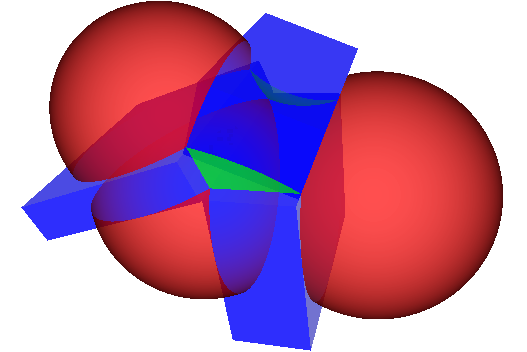
\includegraphics[width=1.5in]{image/obb-tori.png}
  \end{subfigure}
	\caption{Generation of bounding boxes for the SES patches.
	Left: OBBs for spherical triangles.
  Right: OBBs for toroidal patches.}
	\label{fig:obb}
\end{figure}

The ray-casting is implemented using GLSL shaders.
The triangles for the OBB faces are generated on the GPU using a geometry shader.
The OBB is computed from a unit cube for which we compute position, rotation, and scale according to a patch that will by bounded by it.
For a spherical triangle, a cutting plane that contains the triangle's vertices is computed.
Then, the OBB's position, rotation, and scale are computed such that the OBB bounds the smaller part of the sphere when cut by the plane.
Here, we assume that the spherical triangle always fits into a hemisphere.
The OBBs for spherical patches are computed in a similar way.
The difference is in the calculation of the cutting plane.
The plane's normal is computed using midpoints of arcs that bound a patch.
The end points of these arcs are used to position the cutting plane so the half-space defined by it contains all the arc end points.

For the toroidal patches the orientation of their OBBs is computed first.
We compute a vector defined by the centers of the spheres that contain bounding triangles of a toroidal patch.
We use this vector together with the axis of a torus as a second vector to compute a third one -- perpendicular to the two vectors.
These three vectors define the axes of an OBB.
Finally, the extreme points of a patch w.r.t. its OBB orientation are found and the OBB's position and scale are computed based on these points.

In 2013, Kauker et al.~\cite{kauker2013rendering} proposed to ray-cast a toroidal patch using a saddle part of a torus and two clipping planes defined by its delimiting triangles (Fig.~\ref{fig:torus}).
\begin{figure}[htp]
  \centering
  \begin{subfigure}[t]{0.55\columnwidth}
    \centering
    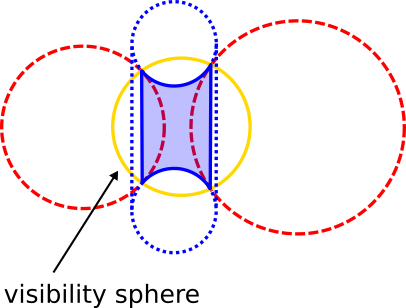
\includegraphics[width=1.7in]{image/torus-vs.png}
    %\caption{Clipping by \textit{visibility sphere}.}
  \end{subfigure}%
  \quad
  \begin{subfigure}[t]{0.4\columnwidth}
    \centering
    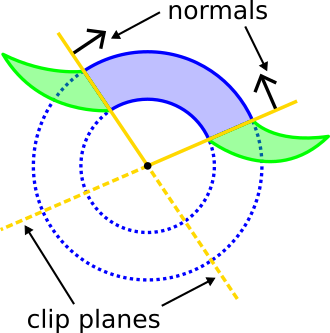
\includegraphics[width=1.3in]{image/torus-planes.png}
    %\caption{Clipping by planes defined by spherical triangles.}
  \end{subfigure}
	\caption{Ray-tracing a toroidal patch. Left: the saddle part of the torus (blue) is cut by the visibility sphere which was introduced in~\cite{krone2009interactive}.
  Right: the patch (blue) is cut from the whole toroidal ring by clipping planes (yellow) defined by the spherical triangles (green).}
	\label{fig:torus}
\end{figure}

We employ this approach and, moreover, we compute these clipping planes for a toroidal patch when writing it into a buffer for ray-casting.
Additionally, we set normals of these clipping planes so that they are facing towards the toroidal patch and we define two types of clipping operations: \textit{AND} and \textit{OR}.
We use these two operations to clip the patches whose angular length around the torus axis is either at most $\pi$ (\textit{AND}) or greater (\textit{OR}).
The \textit{AND} and \textit{OR} operations are defined as their name suggests.
The \textit{AND} operation leaves only fragments that appear on the positive sides of both clipping planes, while the \textit{OR} operation leaves fragments that appear on the positive side of the first or the second clipping plane.
The ray-torus intersection is computed as described by Herbison-Evans~\cite{herbisonevans1995solving}.

%and, moreover, we modify the data structure being used in the original algorithm to store and retrieve all spherical triangles incident to a torus (Fig.~\ref{fig:hashing}). In order to get all neighboring triangles for a torus, we hash the triangles by three keys; i.e., one for each torus which is connected to a triangle.
%For this purpose, we implemented a simple hash table, which is based on linear addressing scheme \cite{alcantara2011efficient}.

%\begin{figure}[htb]
%  \centering
%  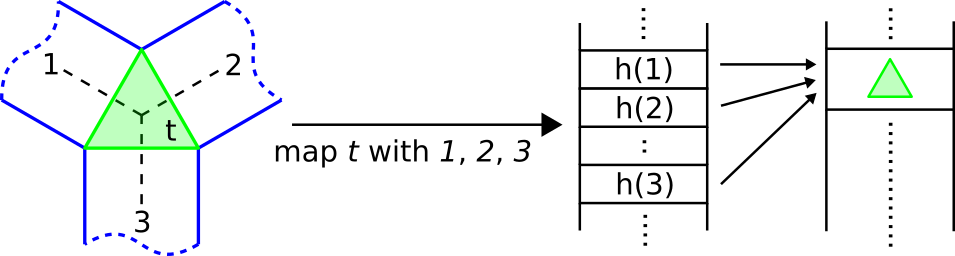
\includegraphics[width=3.3in]{image/hashing.png}
%  \caption{An illustration of the data structure for storing spherical triangles. Triangles $t_1$ and $t_2$ are stored linearly in an array and their incident torus $\tau$ is connected to them using a hash table.}
%	\label{fig:hashing}
%\end{figure}
%This allows us, to ray-cast toroidal patches directly instead of tori.

Ray-casting the sphere is a trivial task. 
However, there can be one or more spherical patches that belong to the same surface atom sphere but they may form different surfaces.
To avoid obvious rendering issues, i.e., distinct coloring, transparency, or visibility, we perform the ray-casting of each patch separately.
%This allows us to visually distinguish between different surface components.
Regarding the separation of patches, we experimented with applying an odd-even rule for polygons~\cite{shimrat1962algorithm} and with computing a convex polyhedron bounds.
We decided for the bounding volume solution because regarding the point-in-polygon (PIP) test there were non-trivial special cases, e.g., a ray going through a polygon's vertex or a very short edge.
These special cases then resulted in pixel artifacts in the final image.
Moreover, the implementation of the PIP test was performance demanding due to many texture memory accesses.
On the other hand, the computation of a patch's bounding volume is based on the fact, that the spherical patch is bounded by planes defined by its bounding arcs.
This way, we have a polyhedron $B_{poly}$ which bounds all the patches belonging to an atom sphere.
For each patch, we add another plane $p_{cut}$ which cuts $B_{poly}$ in order to keep only the volume containing that patch.
$p_{cut}$ is selected as an appropriate plane among planes of the OBB that was used for splatting the patch.
In fact, by splatting, we clip $B_{poly}$ by all the six planes of the OBB.

In the resulting image, there can still occur pixel artifacts caused by numerical issues when ray-casting the tori.
These numerical issues arise when computing an intersection of a ray with a torus.

%\subsection{Ambient Occlusion Opacity Modulation}
%Borland~\cite{borland2011ambient} proposed to utilize ambient occlusion (AO) values to alter the opacity. Motivated by his approach, we exploit the ambient occlusion values as well. Since, we would like to maintain fast rendering performance, we need to remedy the issue of having an object space technique to evaluate the AO values. In the former work of Borland, the performance was considered a less important factor, which allows him to exploit the full object space AO evaluation. Here, we opted for the most recent approach, proposed by Grottel et al.~\cite{grottel2012object}, which renders ambient occlusion values to a $3D$ grid containing an estimate of the volume area of atoms located inside a voxel. Although this approach only reflects the volume of atoms and not the volume area of the molecular surface, we find it as a good trade off between the visual precision and the performance measure. Note, in addition, these values are not employed directly, but rather as opacity modulators instead, which defines the opacity as follows:
%\begin{equation}
  %\alpha = \left( \frac{O}{\tau}\right)^\rho,
	%\label{eq:alpha}
%\end{equation}
%where $\tau$ represents a threshold such that $alpha=1$ if $O\geq\tau$. Moreover, the resulting $\alpha$ values are clampled to interval $[0,1]$. An example of comparison between different $\tau$ values is depicted in Figure~\ref{fig:TODO}.
%
%Another property we propose to use as the opacity modulator is the surface area of the cavity (TODO do we use this as well, or just using colors?).
%\begin{figure}[htb]
%\centering
  %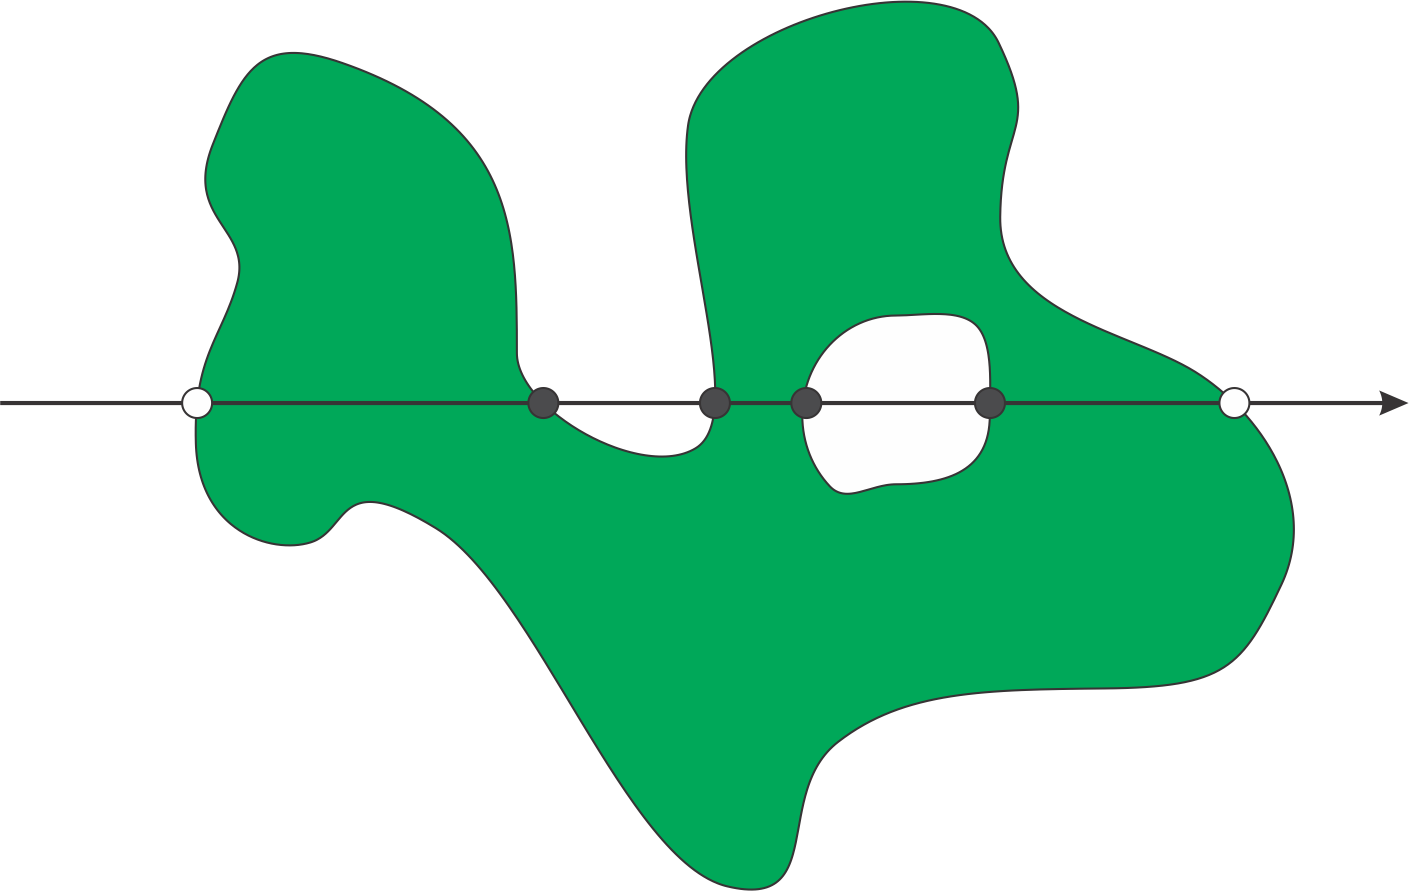
\includegraphics[width=0.8\columnwidth]{image/ray_fragments.png}
  %\caption{(TODO make more nice with overlay AO grid). An example of the list of fragments per a given ray. The color of the circles represent the obtain ambient occlusion value.}
	%\label{fig:ray_fragments}
%\end{figure}

\subsection{Opacity Modulation}\label{sec:opacity}
After the intersection points are computed, we sort them in a front-to-back manner and store them to the linked list. 
Thus, for a given ray, we acquire a list of fragments $\{f_1,\ldots,f_n \}$, where each pair represents an entry and an exit point for the molecular surface. For simplicity, the values of $f_i$ represent the depths of fragments. 
We denote the entire distance the ray passes through the molecule as $l=|f_1-f_n|$. 
As we step along each fragment $f_i$, we define the opacity $\alpha_i$ of even fragments, i.e., those representing the entry surface points, as follows:
\begin{equation}
  \alpha_i = O^{\phi(x)},
	\label{eq:alphaDistEven}
\end{equation}	
where $O$ represents a user-defined parameter affecting the overall opacity and $\phi(x)$ suppress or amplifies the opacity and is defined as
\begin{equation}
  \phi(x) = K-(K-1)x,
	\label{eq:exponent}
\end{equation}	
where $K$ is the maximum value of the exponent and $x=|f_{i+1}-f_i|/l$ represents the ratio of the fragment interval to the entire length $l$. Note that if $x=1$, i.e., having just two fragments on the ray, then $\phi(x)=1$ determining the $\alpha_i=O$. The opacity of odd fragments, i.e., representing the exit surface points, is defined as $\alpha_i = O$, thus keeping them unmodulated since they are less prominent in the final image.
Figure~\ref{fig:Oparam} showcases four different combinations of parameters $K$ and $O$.
\begin{figure*}[htb]
  \centering
  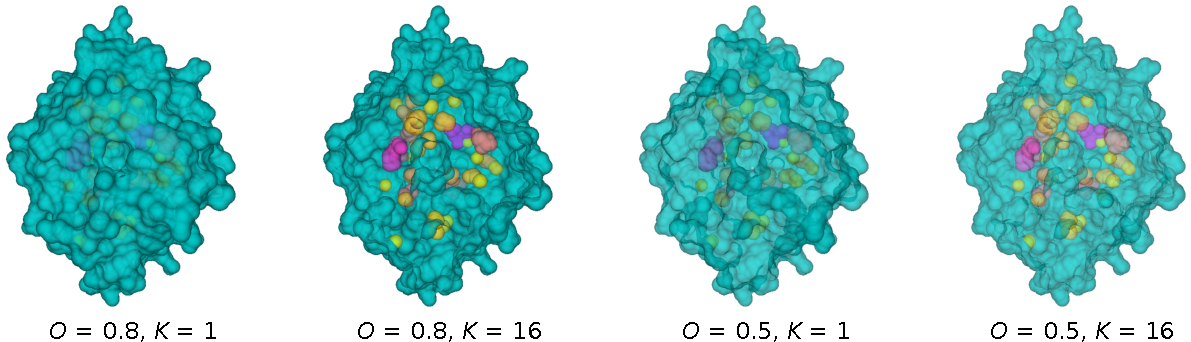
\includegraphics[width=\textwidth]{image/Oparam2.pdf}
  \caption{Example of applying parameters $K$ and $O$ to protein with PDB ID \textit{1CQW}. Note that higher values of the overall opacity $O$ emphasize the front molecular surface, while higher values of maximum exponent $K$ give more prominence to the internal surfaces and cavities.}
	\label{fig:Oparam}
\end{figure*}

\subsection{Cavity Area Estimation}\label{sec:area}
We enhance the visualization of cavities by coloring their surface by their approximate areas.
To estimate the area, we sum the areas of all triangles that form the cavity surface.
The area of a spherical triangle is calculated according to Eq.~\ref{eq:area}:

\begin{equation}
  S = r_{probe}^2 \left[ \left( A + B + C \right) - \pi \right],
	\label{eq:area}
\end{equation}

where $A$, $B$, and $C$ are angles of the triangle. 
%We do the area computation in a GLSL compute shader which computes areas of individual triangles and sums them using atomics.
Additionally, we neglect areas of spherical and toroidal patches since their influence on the exact cavity area is much smaller compared to triangles.
%Therefore, the cavity area we compute is \textcolor{red}{underestimated -- maybe an equation?}.
Naturally, this observation does not hold for the molecular surface.
%\textcolor{red}{What about coloring?}
We also do not handle the case when the triangles intersect each other thus they are clipping themselves.
